\documentclass[12pt,a4paper]{report}
\usepackage[utf8]{inputenc}
\usepackage{amsmath}
\usepackage{amsfonts}
\usepackage{amssymb}
\usepackage{graphicx}
\usepackage[english]{babel}
\usepackage[left=3.50cm, right=2.00cm, top=3.00cm, bottom=3.50cm]{geometry}

\renewcommand{\baselinestretch}{1.5}
\renewcommand{\footnotesize}{\fontsize{13pt}{1}\selectfont}
%\usepackage{sectsty}
%\chapterfont{\centering}

\usepackage{titlesec}
%\titleformat{\chapter}
%{\normalfont\LARGE\bfseries}{\chaptertitlename\ \thechapter}{0.8cm}{}
%\titlespacing*{\chapter}{0pt}{0pt}{20pt}


\usepackage[titletoc]{appendix} 
\usepackage{empheq}
\usepackage{tikz} %draw figure
\usetikzlibrary{shadows,arrows,positioning}
\usepackage{amsthm}             
\usepackage{fancyhdr}
\usepackage{enumitem}
\usepackage{mathtools,etoolbox}
\usepackage{makecell}
\usepackage{tabularx,colortbl}
\usepackage{float} % force the figure to be shown at the location
\usepackage{cases}
\usepackage{tcolorbox}
\usepackage{listings}
\usepackage[nottoc,notlot,notlof]{tocbibind}
\usepackage[driverfallback=hypertex]{hyperref}
\usepackage{url} % hyperref works too
\usepackage[caption = false]{subfig}
\usepackage{longtable}
\usepackage{pgfplots}
\usetikzlibrary{plotmarks}
%\usepackage{wrapfig}
%\usepackage{braket}
%\usepackage{tabto}
%\usepackage{mathrsfs}
%\usepackage{relsize}
%\usepackage{mdframed}
%\usepackage{lipsum}
\usepackage{hyphenat}%prevent hyphenation of table of contents 
\usepackage{color}
\usepackage[final]{pdfpages} % PDF
\urlstyle{same}
\allowdisplaybreaks
\hypersetup{
	colorlinks=true,
	linkcolor=black,
	citecolor=black,
	filecolor=black,
	urlcolor=black,
}
\usepackage{scalefnt}
\definecolor{dkgreen}{rgb}{0,0.6,0}
\definecolor{gray}{rgb}{0.5,0.5,0.5}
\definecolor{mauve}{rgb}{0.58,0,0.82}
\lstset{
	frame=single,
	stringstyle=\color{red},  
%stringstyle=\color{black}, 
	language=Matlab,
	aboveskip=3mm,
	belowskip=3mm,
	showstringspaces=false,
	columns=flexible,
	basicstyle={\small\ttfamily},
	numbers=none,
	numberstyle=\tiny\color{gray},
	keywordstyle=\color{blue},
	commentstyle=\color{dkgreen},
%	keywordstyle=\color{black},
%commentstyle=\color{black},
	breaklines=true,
	%	breakatwhitespace=true,
	tabsize=3
}

\pagestyle{fancy}
\fancyhf{}
\fancyfoot[C]{\thepage}
\lhead{\leftmark}
\fancypagestyle{plain}{%
	\renewcommand{\headrulewidth}{0pt}%
	\fancyhf{}%
	\fancyfoot[C]{\thepage}%
}
\renewcommand{\headrulewidth}{0.4pt}

\graphicspath{{Figure/}} % include path of figure

%% Delimiters
\DeclarePairedDelimiter{\abs}{\lvert}{\rvert}  % abs
\DeclarePairedDelimiter{\norm}{\lVert}{\rVert}  % Norm
\DeclarePairedDelimiter{\inner}{\langle}{\rangle} % Inner product

%% New commands for sets
%\newcommand{\R}{{\mathbb{R}} 


%Theorem
\newtheorem{theorem}{Theorem}[chapter]

\newtheorem{definition}{Definition}[chapter]

\newtheorem{lemma}{Lemma}[chapter]

\newtheorem{remark}{Remark}[chapter]

\newtheorem{proposition}{Proposition}[chapter]

\newtheorem{example}{Example}[chapter]

\newtheorem{properties}{Properties}[chapter]

\newtheorem{corollary}{Corollary}[chapter]

%\newtheorem*{solution}{Solution}


%\newcommand{\theoremautorefname}{Theorem}
\newcommand{\definitionautorefname}{Definition}
\newcommand{\lemmaautorefname}{Lemma}
\newcommand{\remarkautorefname}{Remark}
\newcommand{\propositionautorefname}{Proposition}
\newcommand{\exampleautorefname}{Example}
\newcommand{\propertiesautorefnam}{Properties}
\newcommand{\corollaryautorefnam}{Corollary}
%\newcommand{\solutionautorename}{Solution}

\usepackage{algorithm,algpseudocode,float}
\floatname{algorithm}{Algorithm}
\renewcommand{\algorithmicrequire}{\textbf{INPUT:}}
\renewcommand{\algorithmicensure}{\textbf{OUTPUT:}}

\usepackage[backend = bibtex, sorting = nty, style = ieee]{biblatex}
\addbibresource{References.bib}


\makeatletter
\newenvironment{breakablealgorithm}
{% \begin{breakablealgorithm}
	\begin{center}
		\refstepcounter{algorithm}% New algorithm
		\hrule height.8pt depth0pt \kern2pt% \@fs@pre for \@fs@ruled
		\renewcommand{\caption}[2][\relax]{% Make a new \caption
			{\raggedright\textbf{\ALG@name~\thealgorithm} ##2\par}%
			\ifx\relax##1\relax % #1 is \relax
			\addcontentsline{loa}{algorithm}{\protect\numberline{\thealgorithm}##2}%
			\else % #1 is not \relax
			\addcontentsline{loa}{algorithm}{\protect\numberline{\thealgorithm}##1}%
			\fi
			\kern2pt\hrule\kern2pt
		}
	}{% \end{breakablealgorithm}
		\kern2pt\hrule\relax% \@fs@post for \@fs@ruled
	\end{center}
}
\makeatother

\makeatletter
\newcommand\appendix@chapter[1]{%
	\refstepcounter{chapter}%
	\def\app@ct{Appendix \@Alph\c@chapter: #1}
	\orig@chapter*{\app@ct}%
	\markboth{\MakeUppercase{\app@ct}}{\MakeUppercase{\app@ct}}
	\addcontentsline{toc}{chapter}{\app@ct}%
}
\let\orig@chapter\chapter
\g@addto@macro\appendix{\let\chapter\appendix@chapter}
\makeatother

\makeatletter
\DeclareRobustCommand*{\bfseries}{%
	\not@math@alphabet\bfseries\mathbf
	\fontseries\bfdefault\selectfont
	\boldmath
}
\makeatother


\usepackage{smartdiagram}
\usetikzlibrary{arrows}
\usesmartdiagramlibrary{additions}
\usetikzlibrary{shadows,positioning}
\colorlet{colD}{red!40}
\colorlet{colIP}{cyan!40}
\colorlet{colV}{blue!40}
\colorlet{colBorder}{gray!70}

\tikzset
{mybox/.style=
	{rectangle,rounded corners,drop shadow,minimum height=1cm,
		minimum width=3cm,align=center,fill=#1,draw=colBorder,line width=1pt
	},
	myarrow/.style=
	{draw=#1,line width=3pt,-stealth,rounded corners
	},
	mylabel/.style={text=#1}
}

\smartdiagramset{description title width=2cm, 
	description title text width=1.75cm,
	descriptive items y sep=2,
	description text width=12cm,
	module minimum height=1.4cm,
}

%\usetikzlibrary{shapes.symbols}

\tikzset{description title/.append style={
		signal, 
		signal to=south, 
		signal from=north,
		yshift=-0.65cm,
	}
}

\newcommand{\nocontentsline}[3]{}
\newcommand{\tocless}[2]{\bgroup\let\addcontentsline=\nocontentsline#1{#2}\egroup}
\usepackage{makeidx}

\usepackage{mathrsfs}
\newsavebox\foobox
\newlength{\foodim}
\newcommand{\slantbox}[2][0]{\mbox{%
		\sbox{\foobox}{#2}%
		\foodim=#1\wd\foobox
		\hskip \wd\foobox
		\hskip -0.5\foodim
		\pdfsave
		\pdfsetmatrix{1 0 #1 1}%
		\llap{\usebox{\foobox}}%
		\pdfrestore
		\hskip 0.5\foodim
}}
\def\Laplace{\slantbox[-.45]{$\mathscr{L}$}}

\usepackage{mathabx}

\newsavebox{\accentbox}
\newcommand{\compositeaccents}[2]{%
	\sbox\accentbox{$#2$}#1{\usebox\accentbox}}

\begin{document}
		\thispagestyle{empty}
	\renewcommand{\baselinestretch}{1.2}
	
\begin{center}
	\large{VIETNAM GENERAL CONFEDERATION OF LABOUR} \\
	\large{\textbf{TON DUC THANG UNIVERSITY}} \\
	\large{\textbf{FACULTY OF MATHEMATICS AND STATISTICS}} \\
	\vspace*{1.5cm}
	
	
\includegraphics[scale=0.15]{TDT_logo.jpg} \\
	\vspace*{2cm}
	
	\huge{\textbf{REPORT}} \\ 
	\Huge{\textbf{HAWKES PROCESSES}}\\
	\vspace*{1.5cm}
	
	\LARGE{\textit{by}} \\
	\LARGE{\textbf{Nguyen Le Thao Trang}} \\
	\LARGE{\textbf{Le Thi Minh Phuong}} \\
	\LARGE{\textit{advised by}} \\
	\LARGE{\textbf{Dr. Nguyen Chi Thien}} \\
	\vspace{2cm}
	
%	\Large{\textit{Submitted to the Faculty of Mathematics and Statistics }} \\
%	\Large{\textit{Ton Duc Thang University,}} \\
	\LARGE{\textbf{Course’s Name: Stochastic Processes}} \\
%	\Large{\textbf{Master}} \\
%	\Large{in Applied Mathematics} \\
	
	\vspace{\stretch{1}}
	\large{\textbf{Ho Chi Minh City, Jun 2019}}
	
\end{center}

\newpage
\thispagestyle{empty}
\renewcommand{\baselinestretch}{1.2}

\begin{center}
	\large{VIETNAM GENERAL CONFEDERATION OF LABOUR} \\
	\large{\textbf{TON DUC THANG UNIVERSITY}} \\
	\large{\textbf{FACULTY OF MATHEMATICS AND STATISTICS}} \\
	\vspace*{1.5cm}

	
\includegraphics[scale=0.15]{TDT_logo.jpg} \\
	\vspace*{2cm}

	\huge{\textbf{REPORT}} \\ 
	\Huge{\textbf{HAWKES PROCESSES}}\\
	\vspace*{1.5cm}

	\LARGE{\textit{by}} \\
	\LARGE{\textbf{Nguyen Le Thao Trang}} \\
	\LARGE{\textbf{Le Thi Minh Phuong}} \\
	\LARGE{\textit{advised by}} \\
	\LARGE{\textbf{Dr. Nguyen Chi Thien}} \\
	\vspace{2cm}

	%	\Large{\textit{Submitted to the Faculty of Mathematics and Statistics }} \\
	%	\Large{\textit{Ton Duc Thang University,}} \\
	\LARGE{\textbf{Course’s Name: Stochastic Processes}} \\
	%	\Large{\textbf{Master}} \\
	%	\Large{in Applied Mathematics} \\

	\vspace{\stretch{1}}
	\large{\textbf{Ho Chi Minh City, Jun 2019}}
	
\end{center}

	\newpage
	\thispagestyle{empty}
	\renewcommand{\baselinestretch}{1.2}
	\begin{center}
		\Large{\textbf{ACKNOWLEDGMENT}} \\
	\end{center}
	Foremost, we would like to express our sincere gratitude to our advisor Dr. Nguyen Chi Thien for his guidance, encouragement, enthusiasm, and patience. His guidance helped us to learn a lot of things that we had not previously known. The knowledge that we received not only helped and facilitated our completion of the report but also gave us the good experience in the future.  We are also thankful for his useful comments and hard questions for our study. Thank you so much for everything that you give us, Dr. Thien.
	\\
	Besides our advisor, we would like to thank Ton Duc Thang University and Faculty of Mathematics and Statistics and Information Technology, for providing us both the good learning environment and modern facilities to complete report, and the opportunity to work together and meet many interesting people.
	\\
	We would like to thank family and friends who supported us during our study at Ton Duc Thang University, for all their love, concern, advice and help when we need them. 
	%	We are indebted to them for all their help.
	\\
	Finally thank you everyone. Thank you very much!
	\newpage
	\thispagestyle{empty}
	\renewcommand{\baselinestretch}{1.2}
\begin{center}
	\Large{\textbf{THE REPORT HAS BEEN ACCOMPLISHED}} \\
	\Large{\textbf{AT TON DUC THANG UNIVERSITY}} \\
\end{center}

	We hereby declare that this report was carried out by ourselves under the guidance and supervision of Dr. Nguyen Chi Thien; and that the work contained and the results in this report are true and have not been either submitted anywhere for any previous purpose or published in any other literature. The data and figures presented in this report are for analysis, comments, and evaluations from various resources by our own work and have been fully acknowledged in the reference part.
	In addition, other comments, reviews and data from other authors, and organizations used in this report have been acknowledged, and explicitly cited.
	We will take full responsibility for any fraud detected in our report. Ton Duc Thang University is unrelated to any copyright infringement caused on our work (if any). \\
	
	\begin{flushright}
		Ho Chi Minh City, Jun 2019 \hspace*{1cm} \\
		Student 1 \hspace*{2.5cm} \\
		\vspace*{2cm}
		Nguyen Le Thao Trang \hspace*{1.2cm} \\
		Student 2 \hspace*{2.5cm} \\
		\vspace*{2cm}
		Le Thi Minh Phuong \hspace*{1.5cm}
	\end{flushright}

	\tableofcontents 
	\thispagestyle{empty}
	\addtocontents{toc}{\protect\thispagestyle{empty}}

%	\listoftables
%	\thispagestyle{empty}

	\listoffigures
	\thispagestyle{empty}
    \addtocontents{lof}{\protect\thispagestyle{empty}}
	

	\listofalgorithms
	\thispagestyle{empty}
	
	\newpage
	\pagenumbering{arabic}

	\chapter{Introduction}
\label{chapter:intro}
In reality, an earthquake can increase the geological tension in the region where it occurs. Selling a significant quantity of a stock could cause a trading flurry. These above problems are called the applications of self-exciting stochastic processes. This process is called Hawkes process which was proposed by Alan G. Hawkes \cite{hawkes}. \\
The Hawkes process is a counting process that models a sequence of 'arrivals' of some types over time, for example, earthquakes, trade orders. Each arrival excites the process, i.e., the chance of a next arrival is increased for some time period after the initial arrival.\\
%and it is based on a counting process in which the intensity function depends explicitly an all previously occurred events. 
The outline of this report is organized as follows:

	Chapter \ref{chapter:knowledge} reviews and introduces some basis knowledge. It will support us in the next chapters such as point process, counting process, conditional intensity function, inhomogeneous Poisson process.
	
	Chapter \ref{chapter:hawkes} approaches two models to simulate Hawkes process: the intensity-based Hawkes process and cluster-based Hawkes process.
	
	Chapter \ref{chapter:simulation} is devoted to some simulations by using Matlab\textsuperscript{\textregistered} code such as the inhomogeneous Poisson process and intensity-based Hawkes process and cluster-based Hawkes process.
	
	Chapter \ref{chapter:application} will introduce an application of Hawkes process in seismology.
	
	Chapter \ref{chapter:conclusion} summarizes the content of the report what has been done and limited of its.\\
%	summarizes the thesis and analysisnof the results. We also discuss how to apply the method to other applications.
	
	\chapter{Knowledge}
\label{chapter:knowledge}
In order to clearly understand the Hawkes process, we will introduce the definition of point process, counting process and conditional intensity function. And then we discuss the  inhomogeneous Poisson process. It is necessary to discuss because one can view the Hawkes process as a generalization of the (time) inhomogeneous Poisson process.
\section{Point process and counting process}
\begin{definition}
	\cite{hawkes} \textbf{(Point process)} Let $\{T_i, i \in \mathbb{N} \}$ be a sequence of non-negative random variables such that $\forall i \in \mathbb{N}, T_i<T_{i+1}$. Then $\{T_i, i \in \mathbb{N} \}$ is a (simple) point process.
\end{definition}
\begin{definition}
	\cite{hawkes} \textbf{(Counting process)} A counting process is a stochastic process $(N(t):t \geq 0)$ taking values in $\mathbb{N}_0$ that satisfies $N(0)=0$, is almost surely finite, and is a right-continuous step function with increments of size +1. Denote by $(\mathcal{H}(u): u \geq 0)$ the history of the arrivals up to time $u$.
\end{definition}
\noindent
For example:
\begin{itemize}
	\item If $N(t)$ is the number of persons who enter a store by time $t$, then $(N(t):t \geq 0)$ is a counting process in which an event corresponds to a person enters the store.
	\item If $N(t)$ is the number of goals that a given football player scores by time $t$ , then $(N(t):t \geq 0)$ is a counting process in which an event of the process will occur whenever the football player scores a goal.
\end{itemize}
\begin{figure}[H]
	\centering
	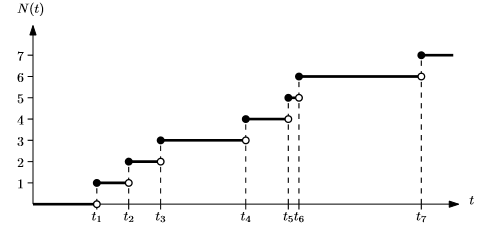
\includegraphics{coutingprocess}
	\caption[Point process $\{t_1, t_2,...\}$ and corresponding counting process $N(t)$.]{Point process $\{t_1, t_2,...\}$ and corresponding counting process $N(t)$.}
\end{figure}
\section{Conditional intensity function}
It is difficult to work with the conditional arrival distribution $f^*(t)$, so one used another characterization of point process which was called conditional intensity function. This function is defined in the form
\begin{align*}
	\lambda^*(t)=\dfrac{f^*(t)}{1-F^*(t)}
\end{align*}
where $f^*(t)$ is the conditional probability density function (p.d.f) of the next arrival given the previous arrival history and $F^*(t)$ is the cumulative distribution function (c.d.f) of the next arrival given the previous arrival history.
\begin{definition}
	\label{def:cif}
	\cite{hawkes} \textbf{(Conditional intensity function)} Consider a counting process $N(.)$ with associated histories $\mathcal{H(.)}$. If a function $\lambda^*(t)$ exists such that
	\begin{align*}
		\lambda^*(t) = \lim_{h\downarrow 0} \frac{\mathbb{E}[N(t + h) - N(t)|\mathcal{H}(t)]}{h}
	\end{align*}
	which only relies on information of $N(.)$  in the past (that is, $\lambda^*(t)$ is $\mathcal{H}(t)$ - measurable), then it is called the conditional intensity function of $N(.)$.
\end{definition}
\begin{figure}[H]
	\centering
	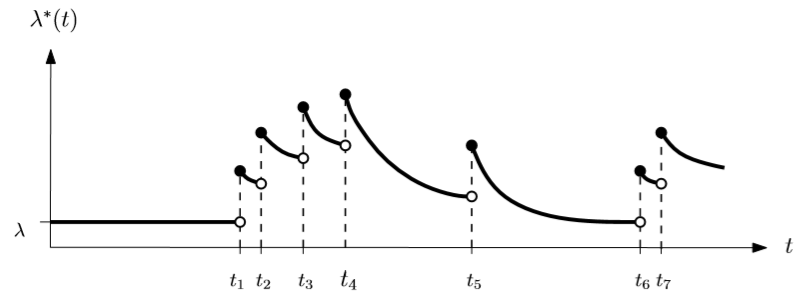
\includegraphics[scale=.75]{conditionintensityfunction}
	\caption[The conditional intensity function for a self-exciting process.]{The conditional intensity function for a self-exciting process.}
\end{figure}
\section{Inhomogeneous Poisson process}
\subsection{Description}
The inhomogeneous Poisson process is a generalization of the homogeneous Poisson process that intensity function depends on the time $t$.
\begin{definition}
	\textbf{(Inhomogeneous Poisson Process)} Consider $(N(t):t \geq 0)$ a counting process, that satisfies
	\begin{align*}
	\mathbb{P}(N(t+h)-N(t)=m|N(t))=
	\begin{cases}
	\lambda(t)h,& \text{if } m=1\\
	o(h) ,& \text{if } m>1\\
	1-\lambda(t)h+o(h),& \text{if } m=0
	\end{cases}
	\end{align*}
	Then a counting process $N(t)$ is called an inhomogeneous Poisson process with an intensity function $\lambda:\mathbb{R}^+ \rightarrow \mathbb{R}^+$.
\end{definition}
The intensity function $\lambda(t)$ of an inhomogeneous Poisson process is a deterministic function.
\begin{definition} \cite{thesis} \textbf{(Mean Value Function)} The function 
	\begin{align*}
	m(t) = \int_{0}^{t} \lambda(y)dy
	\end{align*}
	is called the mean value function of the inhomogeneous Poisson process.
\end{definition}
\begin{theorem}
	\cite{thesis} If $\{ N(t), t \geq 0\}$ is a non-stationary Poisson process with intensity function $\lambda(t), t \geq 0$, then $N(t + h) - N(h
	)$ is a Poisson random variable with mean $m(t + h) - m(h) = \displaystyle\int_{h}^{h + t}\lambda(y)dy$.
\end{theorem}
\subsection{The algorithm}
The idea of this algorithm is to generate a homogeneous Poisson process, and then remove the points probabilistically so that the remaining points satisfy the time-varying intensity $\lambda(.)$. This algorithm requires the conditional intensity to be upper bounded, i.e., $\exists M$ such that $\lambda(.) \leq M$ on $[0,T]$.
\begin{breakablealgorithm}
	\caption{Generate an inhomogeneous Poisson process by thinning.}
	\label{algorithm:poison}
	\begin{algorithmic}[H]
		\noindent
		\algorithmicrequire{ $T$ is the time to simulate; \\
			\hspace*{1.8 cm}$\lambda(.)$ is the intensity function; \\
			\hspace*{1.7 cm}$M$ is upper bounded value;}\\
		\algorithmicensure{ Retrieve the simulated process $\{t_1, t_2,...,t_n\}$ on $[0,T]$;}\\
%		\algorithmicensure{ The vector $P$ containing the times of occurrences $\{t_1, t_2,...,t_n\}$;}\\
		\textbf{Require:} $\lambda(.) \leq M$ on $[0,T]$.\\
		\begin{itemize}
			\item [1.] $P\leftarrow []$, $t\leftarrow0$
			\item [2.] \textbf{while} $t<T$ \textbf{do}
			\item [3.] \hspace*{.6cm}Generate next candidate point: $E \leftarrow$ Exp $(M)$,  $t \leftarrow t+E$
			\item [4.] \hspace*{.5cm} Keep it with some probability:  $U \leftarrow$ Unif$(0,M)$
			\item [5.] \hspace*{.55cm} \textbf{if} $t <T$ \textbf{and} $U \leq \lambda(t)$ \textbf{then}
			\item [6.]  \hspace*{1.2cm}$P \leftarrow [P,t]$
			\item [7.] \hspace*{.65cm}\textbf{end if}
			\item [8.] \textbf{end while}
		\end{itemize}
	\end{algorithmic} 
\end{breakablealgorithm}


	\include{Hawkes}
	\chapter{Simulation Algorithms}
\label{chapter:simulation}
In this chapter, we will give some simulations in  Matlab\textsuperscript{\textregistered} environment: Inhomogeneous Poisson Process, Intensity-based Hawkes Process, Cluster-based Hawkes Process.
\section{Simulation of Inhomogeneous Poisson Process}
The Inhomogeneous Poisson Process is given in Algorithm \ref{algorithm:poison} that is performed Matlab\textsuperscript{\textregistered} environment.
\lstinputlisting{InhomogeneousPoissonProcess.m}
\begin{example}
	\label{example:inhomogeneouspoi}
 Simulating an inhomogeneous Poisson process with intensity function $\lambda(t)=2+\sin(t)$, bounded value $M=4$ and $T=4\pi$.
\end{example}
%To simulate in the \autoref{example:inhomogeneouspoi}, we will call function as follows:
%\lstinputlisting{main_InhomogeneousPoissonProcess.m}
\begin{figure}[H]
	\centering
	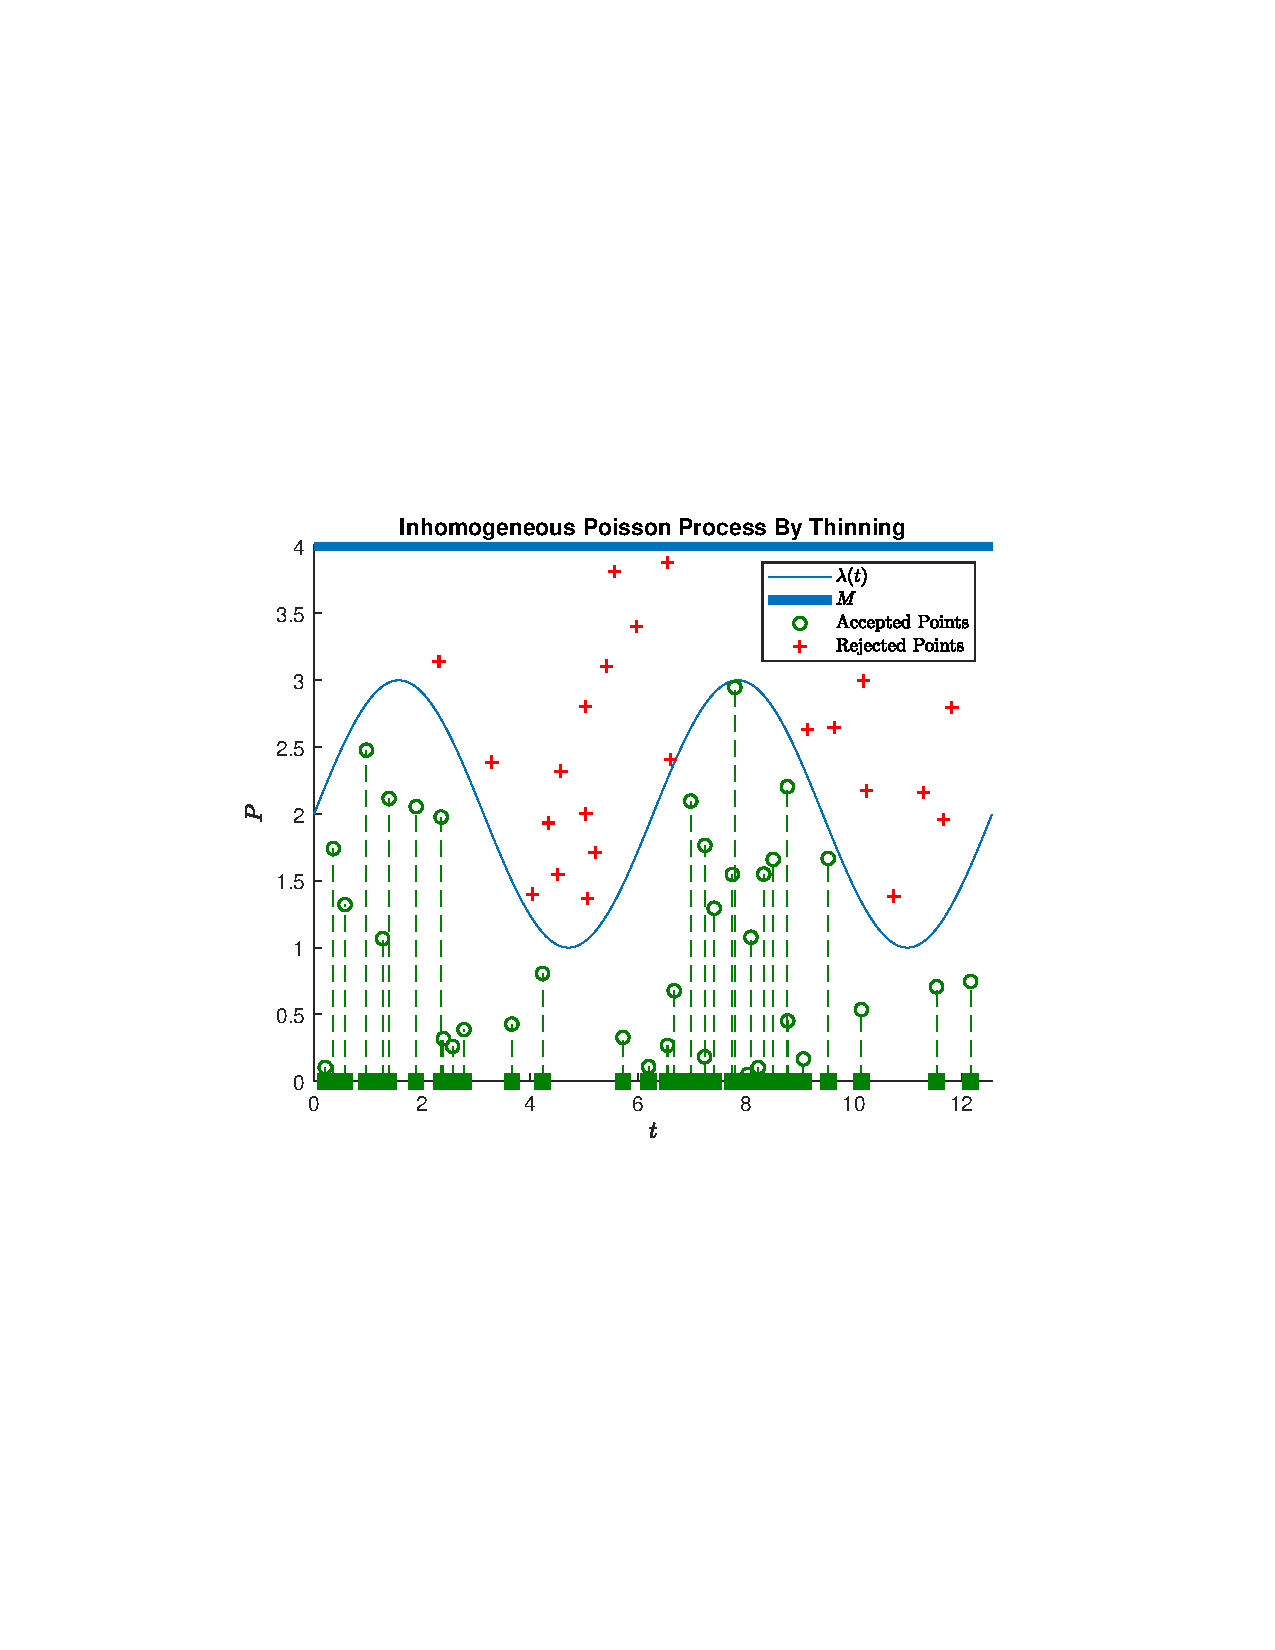
\includegraphics[trim={5cm 9cm 3.5cm 9cm},height=4.5in,width=6.5in]{inhomopoisson.pdf}
	\caption[The inhomogeneous Poisson process.]{The inhomogeneous Poisson process.}
	\label{figure:inhomopoisson}
\end{figure}
Figure \ref{figure:inhomopoisson} illustrates the result of inhomogeneous Poisson process. Each $(t,P)$ point describes a proposed arrival at time $t$ whose $P$ value. The circles are the accepted points, the plus signs are the rejected points and the squares are the point processes.
\section{Simulation of Intensity-based Hawkes Process}
The Intensity-based Hawkes Process is given in Algorithm \ref{algorithm:hawkesthinning} that is performed Matlab\textsuperscript{\textregistered} environment.
\lstinputlisting{HawkesProcessByThinning.m}
\lstinputlisting{cif.m}
\begin{example}
	\label{example:hawkesthinning}
	Simulating a intensity-based Hawkes Process with condition intensity function $(\lambda,\alpha,\beta)=(1,1,1.2)$ and $T=4$.
\end{example}
Figure \ref{figure:hawkesthinning} illustrates the result of the Intensity-based Hawkes Process in the \autoref{example:hawkesthinning}. Each $(t,P)$ point describes a proposed arrival at time $t$ whose $P$ value. The circles are the accepted points, the plus signs are the rejected points and the squares are the point processes.
%\textbf{Solution}
%To simulate in the \autoref{example:hawkesthinning}, we will call function as follows:
%\lstinputlisting{main_HawkesProcessByThinning.m}
\begin{figure}[H]
	\centering
	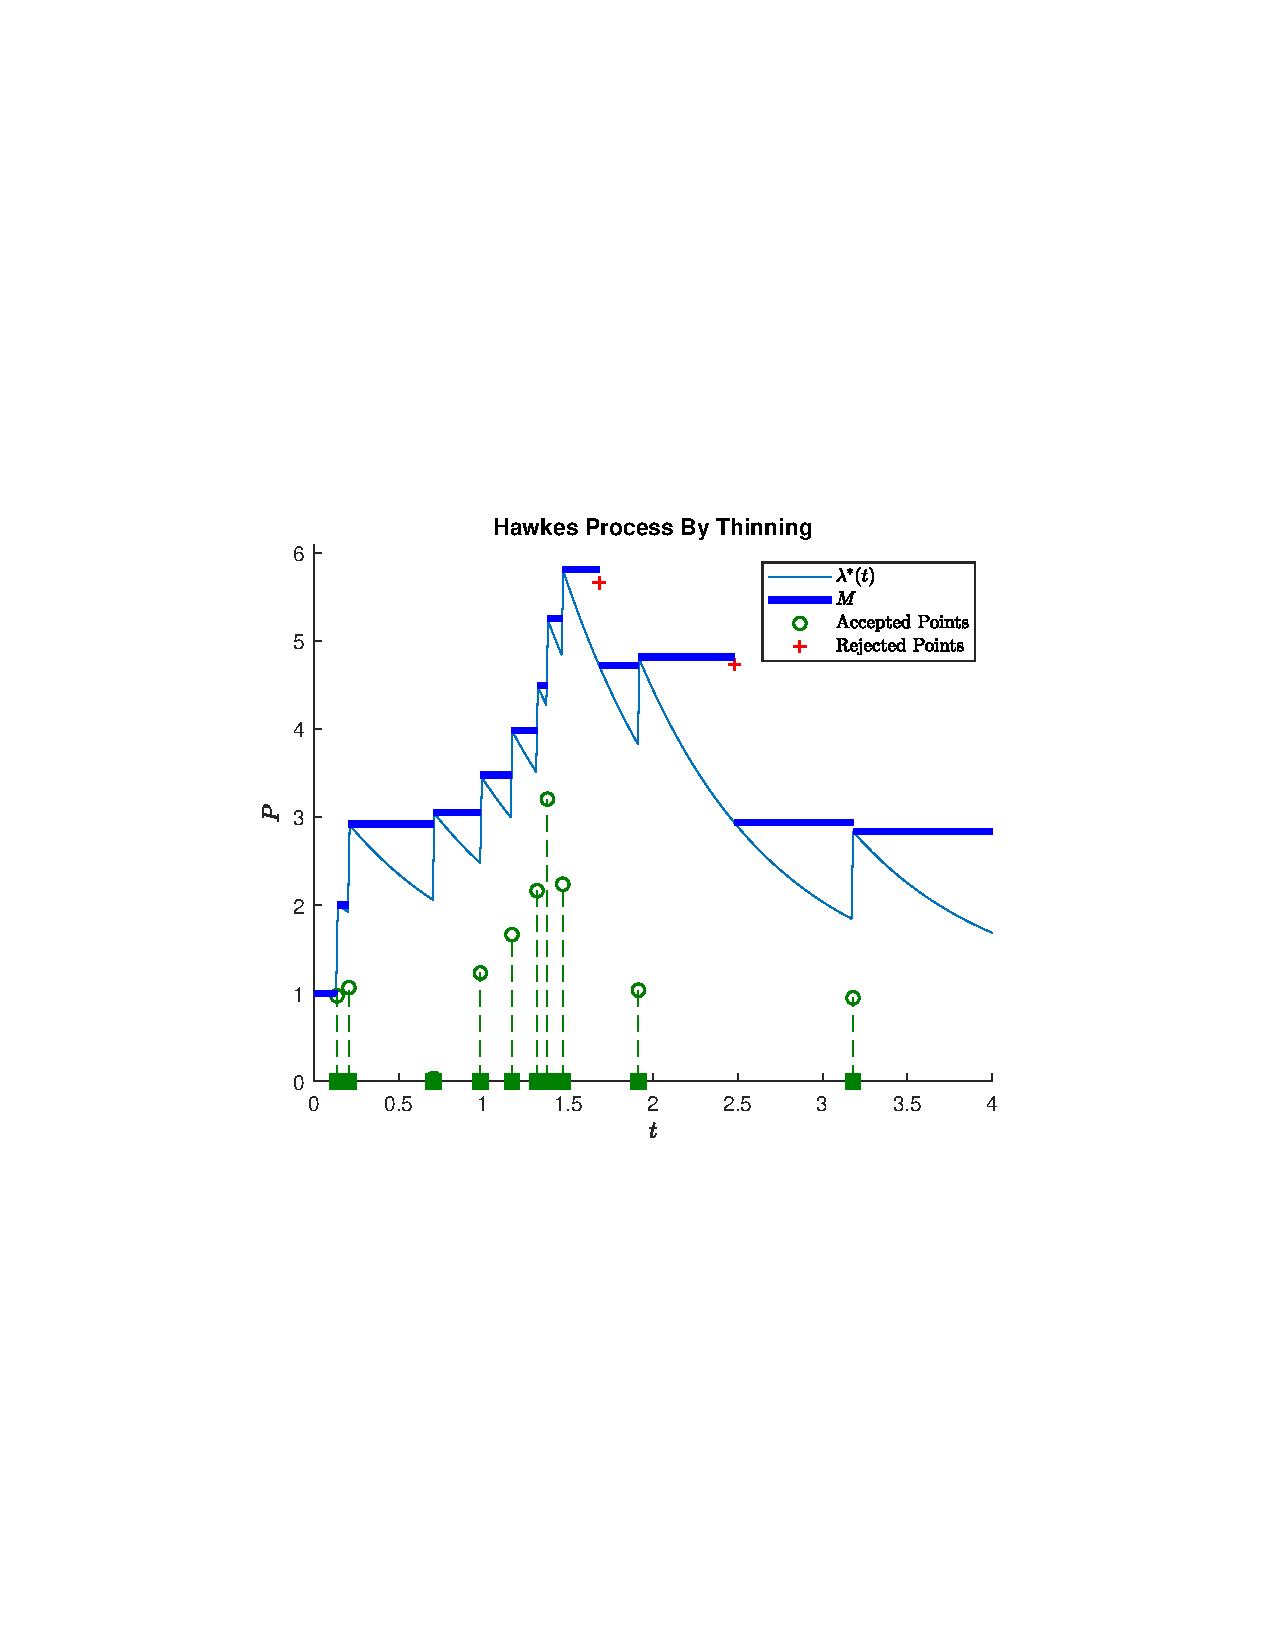
\includegraphics[trim={5cm 9cm 3.5cm 9cm},height=4.5in,width=6.5in]{hawkesbythinning.pdf}
	\caption[The Intensity-based Hawkes Process.]{The Intensity-based Hawkes Process.}
	\label{figure:hawkesthinning}
\end{figure}
\section{Simulation of Cluster-based Hawkes Process}
The Cluster-based Hawkes Process is given in Algorithm \ref{algorithm:hawkescluser} that is performed Matlab\textsuperscript{\textregistered} environment.
\lstinputlisting{HawkesProcessByClustering.m}
\begin{example}
	\label{example:hawkescluster}
	Simulating a cluster-based Hawkes Process with condition intensity function $(\lambda,\alpha,\beta)=(1,2,1.2)$ and $T=10$.
\end{example}
%\textbf{Solution}
%To simulate in the \autoref{example:hawkescluster}, we will call function as follows:
%\lstinputlisting{main_HawkesProcessByClustering.m}
\begin{figure}[H]
	\centering
	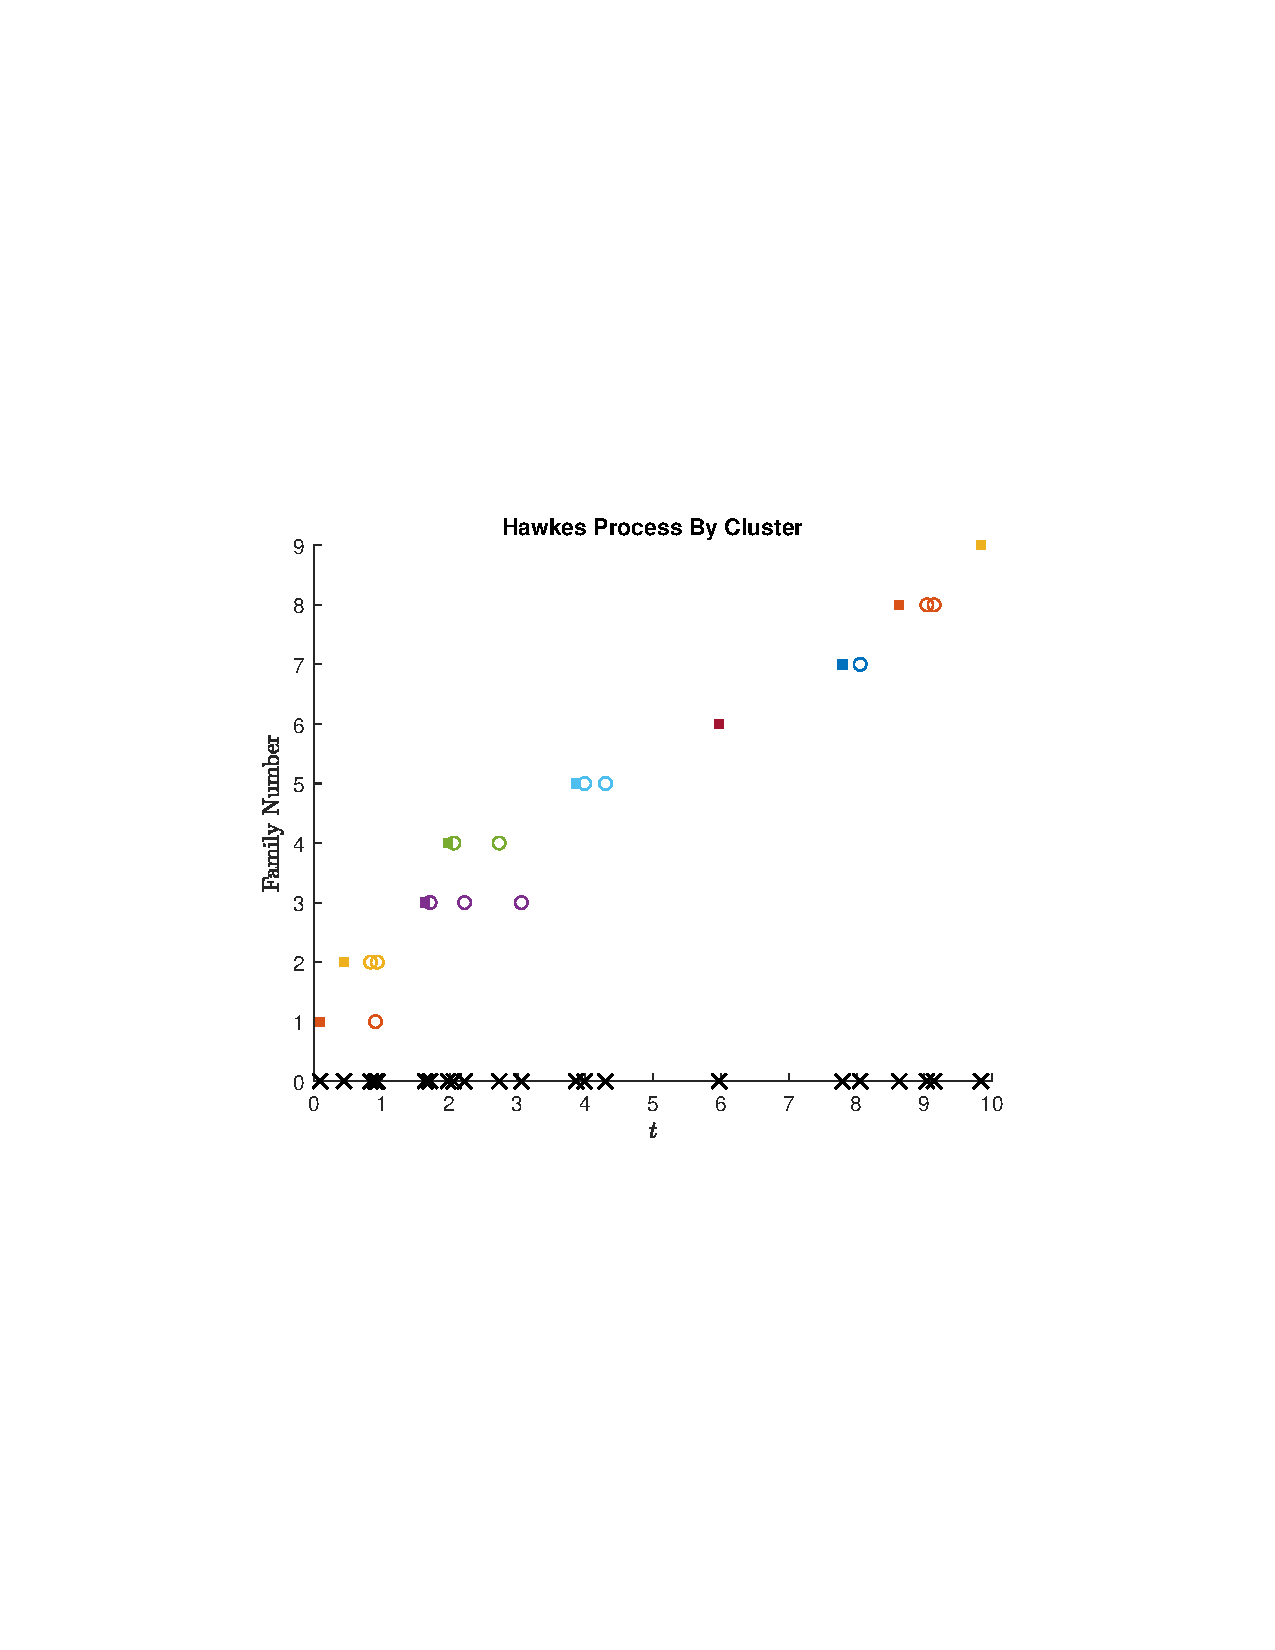
\includegraphics[trim={5cm 8.8cm 3.5cm 9cm},height=4.5in,width=6.5in]{hawkesbycluster.pdf}
	\caption[The Cluster-based Hawkes Process.]{The Cluster-based Hawkes Process.}
	\label{figure:hawkescluster}
\end{figure}
Figure \ref{figure:hawkescluster} illustrates the result of the Cluster-based Hawkes Process. The squares are the immigrant points, the circles of the same height and color are descendant of immigrant points and the crosses are the point processes.
	\chapter{An application of Hawkes process}
\label{chapter:application}
In reality, a Hawkes processes have been applied in many areas from earthquake to financial analysis. In this chapter, we introduce an application of Hawkes process in seismology.\\
In the 1970s, professor Alan Hawkes introduced a mathematical model of self-exciting process in seismology, which is called Hawkes process. And then it was expanded by Y.Ogata and L.Adamopoulos. In \autoref{figure:earth} illustrates the number of shocks in periods of three months for an area of the North Atlantic as same as the stochastic intensity function of a Hawkes process. Therefore, the ETAS model was introduced to modeling the earthquake times and magnitudes \cite{thesis}. They are given as follows:
\begin{align*}
	\lambda(t) = \lambda_0 + \alpha \sum_{T_i < t}e^{\beta \kappa_i}e^{-\delta(t - T_i)},
\end{align*}
where $\kappa_i \in [0, \infty)$ is the magnitude of an earthquake occurring at time $T_i$ and $\alpha , \beta, \delta > 0$ are parameters. In case 
\begin{align*}
	f(\kappa| t) = \gamma e^{-\gamma t}
\end{align*}
Additional, we can define it by its conditional intensity function including both marks and times
\begin{align*}
	\lambda(t, \kappa) = (\lambda_0 + \alpha \sum_{T_i < t}e^{\beta \kappa_i}e^{-\delta(t - T_i)})\gamma e^{-\gamma t}
\end{align*}  
The idea of this model is that earthquakes cause aftershocks, large earthquakes increase the intensity more than small earthquakes. 
\begin{figure}[H]
	\centering
	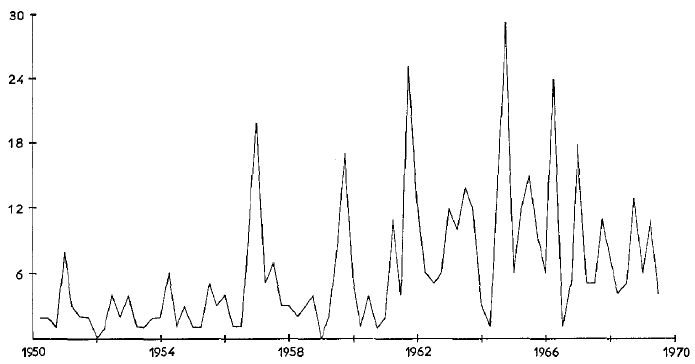
\includegraphics[width=5in]{earthquakes}
	\caption[Number of shocks in periods of three months for area of North Atlantic.]{Number of shocks in periods of three months for area of North Atlantic \cite{thesis}.}
	\label{figure:earth}
\end{figure}
	\chapter{Conclusion}
\label{chapter:conclusion}
In this report, we have studied Hawkes process is a self-exciting stochastic process, which based on a counting process in which the intensity function depends on all previously occurred events. 

In the Chapter \ref{chapter:knowledge}, we have reviewed some basis knowledge such as point process, counting process, conditional intensity function, inhomogeneous Poisson process to apply for analysis of the Hawkes process.

In the Chapter \ref{chapter:hawkes}, we have studied two models to simulate Hawkes process: the intensity-based Hawkes process Model and cluster-based Hawkes process Model.

In the Chapter \ref{chapter:simulation}, we have simulated three algorithms such as inhomogeneous Poisson process, Intensity-based Hawkes Process and Cluster-based Hawkes Process in Matlab\textsuperscript{\textregistered} environment.

In the Chapter \ref{chapter:application}, we have studied an application of Hawkes process in seismology.\\
Currently, we only simulate one dimensional Hawkes processes. However, we can extend to simulate the multidimensional Hawkes processes in the future. This is a limitation of this report. 
	
	\renewcommand{\bibname}{References}
	\addcontentsline{toc}{chapter}{References}
	\printbibliography
\end{document}